% !TEX spellcheck = en_US



% ~~~~~~~~~~~~~~~~~~~~~~~~~~~~~~~~~~~~~~~ V
% (NC) 2026 Haluk Bingol
% github.com/halukbingol/LaTeX-Templates
%
% Licensees may copy, distribute, display, and perform the work and make derivative works 
% and remixes based on it only for non-commercial purposes. 
% ~~~~~~~~~~~~~~~~~~~~~~~~~~~~~~~~~~~~~~~ A




% =====================================================================
%  The Eclipse IDE -- Senior Level: Architecture, the Compiler as a Library, Team Setups and Security
%  ---------------------------------------------------------------------
%  Built on hblib/Template/hblibTemplate.tex with the libraries in ../../hblib/.
%  Programs and their real outputs are in codeoutput/:
%     codeoutput/<Name>.java  a program (classes without main() are only compiled)
%     codeoutput/<Name>.sh    a terminal session, run in a copy of codeoutput/<Name>/
%     codeoutput/<Name>.txt   what it printed, made by:  bash run_examples.sh
% =====================================================================

\documentclass[aspectratio=169,10pt,compress]{beamer}

% ~~~~~~~~~~~~~~~~~~~~~~~~~~~~~~~~~~~~~~~~~~~~~~~~~~~~~~~~~~~~~~~~~ V hblib
	\usepackage{../../hblib/hblibPresentation} % lib presentation: theme, i/N, \hSection, algorithm2e, ...
	\usepackage{../../hblib/hblibCodeoutput} % lib code + output: \lstcode, \lstterminal, ...
	\usepackage{../../hblib/hblibDatastructures} % lib data structures: \hString, \hStack, \hQueue
% ~~~~~~~~~~~~~~~~~~~~~~~~~~~~~~~~~~~~~~~~~~~~~~~~~~~~~~~~~~~~~~~~~ A hblib


% theme, i/N, fonts (T1, lmodern), booktabs, xcolor, array (L{width} columns), listings, tikz,
% algorithm2e (\small captions, \Fn) and the color gitred come from the hblib libraries




% +++++++++++++++++++++++++++++++++++++++ V specific
\DontPrintSemicolon % in algorithms
\newcommand{\win}{\textbf{Windows}}
\newcommand{\mac}{\textbf{macOS}}
% +++++++++++++++++++++++++++++++++++++++ A specific

% ---------------------------------------------------------------------
\title{The Eclipse IDE}
\subtitle{Senior Level: Architecture, the Compiler as a Library, Team Setups and Security}
\author[Bingol]{Haluk O. Bingol}

\institute[FCIS]{
    Faculty of Computer and Information Sciences\\
    Yeditepe University
}
\date{
	{\tiny \hbTimeStamp}
}

\begin{document}




% ~~~~~~~~~~~~~~~~~~~~~~~~~~~~~~~~~~~~~~ V frm
\begin{frame}[t,fragile]
  \titlepage
\end{frame}
% ~~~~~~~~~~~~~~~~~~~~~~~~~~~~~~~~~~~~~~ A frm




% ~~~~~~~~~~~~~~~~~~~~~~~~~~~~~~~~~~~~~~ V frm
\begin{frame}[t,fragile] \frametitle{Outline}
  \begin{columns}[T]
    \begin{column}{0.48\textwidth}
      \tableofcontents[sections={1-4}, hideallsubsections]
    \end{column}
    \begin{column}{0.48\textwidth}
      \tableofcontents[sections={5-7}, hideallsubsections]
    \end{column}
  \end{columns}
\end{frame}
% ~~~~~~~~~~~~~~~~~~~~~~~~~~~~~~~~~~~~~~ A frm

% ~~~~~~~~~~~~~~~~~~~~~~~~~~~~~~~~~~~~~~ V
\hSection[Architecture]{Bundles and Extension Points}
% ~~~~~~~~~~~~~~~~~~~~~~~~~~~~~~~~~~~~~~ A




% ~~~~~~~~~~~~~~~~~~~~~~~~~~~~~~~~~~~~~~ V frm
\begin{frame}[t,fragile] \frametitle{OSGi: an IDE made of bundles}
  \begin{columns}[T]
    \begin{column}{0.5\textwidth}
      \begin{itemize}\small
        \item A \textbf{bundle} (plug-in) is a JAR with extra headers in \texttt{META-INF/MANIFEST.MF}: name, version,
              which packages it \textbf{exports}, which bundles it \textbf{requires}.
        \item The OSGi runtime (Equinox) gives every bundle its own class loader: a bundle sees only what others export.
        \item Bundles start \textbf{lazily}: the Java tools are not loaded until you open a Java file.
        \item \textbf{p2} installs and updates bundles from update sites (Marketplace, \menu{Help > Install New Software\dots}).
      \end{itemize}
    \end{column}
    \begin{column}{0.46\textwidth}
      \begin{center}
      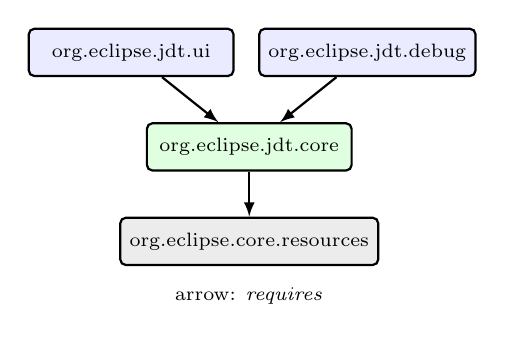
\begin{tikzpicture}[b/.style={draw, thick, rounded corners=2pt, minimum width=2.6cm, minimum height=0.6cm, font=\scriptsize, fill=blue!8}]
        \node[b] (ui)  at (0,2.4) {org.eclipse.jdt.ui};
        \node[b] (dbg) at (3,2.4) {org.eclipse.jdt.debug};
        \node[b, fill=green!12] (core) at (1.5,1.2) {org.eclipse.jdt.core};
        \node[b, fill=gray!15]  (res)  at (1.5,0)   {org.eclipse.core.resources};
        \draw[-latex, thick] (ui) -- (core); \draw[-latex, thick] (dbg) -- (core); \draw[-latex, thick] (core) -- (res);
        \node[font=\scriptsize] at (1.5,-0.7) {arrow: \emph{requires}};
      \end{tikzpicture}
      \end{center}
    \end{column}
  \end{columns}
\end{frame}
% ~~~~~~~~~~~~~~~~~~~~~~~~~~~~~~~~~~~~~~ A frm




% ~~~~~~~~~~~~~~~~~~~~~~~~~~~~~~~~~~~~~~ V frm
\begin{frame}[t,fragile] \frametitle{A real bundle: JDT Core, the Java model and compiler}
  \lstterminal[basicstyle=\ttfamily\tiny]{codeoutput/Bundle.txt}

  \vspace{0.1em}
  \small
  The JDT Core JAR is a normal JAR \emph{and} a bundle (this one is from Eclipse 4.26; 2026-06 has a newer version of the same bundle).
  \texttt{plugin.xml} declares \textbf{extension points}: places where other bundles can plug in.
\end{frame}
% ~~~~~~~~~~~~~~~~~~~~~~~~~~~~~~~~~~~~~~ A frm




% ~~~~~~~~~~~~~~~~~~~~~~~~~~~~~~~~~~~~~~ V frm
\begin{frame}[t,fragile] \frametitle{Extension points}
  \begin{columns}[T]
    \begin{column}{0.52\textwidth}


% +++++++++++++++++++++++++++++++++++++++ V lst
%: -Lst.
\begin{lstlisting}[style=codesnippet, language=XML, basicstyle=\ttfamily\tiny]
<!-- plugin.xml of a plug-in that adds a quick fix -->
<extension point="org.eclipse.jdt.ui.quickFixProcessors">
  <quickFixProcessor
      id="tr.edu.yeditepe.fixes.turkishI"
      name="Turkish i fixes"
      class="tr.edu.yeditepe.fixes.TurkishIProcessor"/>
</extension>
\end{lstlisting}
% +++++++++++++++++++++++++++++++++++++++ A lst


      \small \hRemark{Not run here}: needs the Eclipse SDK (Plug-in Development Environment).
    \end{column}
    \begin{column}{0.44\textwidth}
      \begin{itemize}\small
        \item A bundle \textbf{declares} an extension point (an XML schema); others \textbf{contribute} extensions.
        \item Eclipse reads the XML at start without loading the classes: thousands of contributions cost little.
        \item Menus, views, editors, builders, quick fixes, launchers: all are extensions.
        \item Build plug-ins with \texttt{File > New > Plug-in Project} (\emph{Eclipse IDE for RCP and RAP Developers} or
              \emph{Eclipse SDK}).
      \end{itemize}
    \end{column}
  \end{columns}
\end{frame}
% ~~~~~~~~~~~~~~~~~~~~~~~~~~~~~~~~~~~~~~ A frm

% ~~~~~~~~~~~~~~~~~~~~~~~~~~~~~~~~~~~~~~ V
\hSection[Compiler]{The Compiler as a Library}
% ~~~~~~~~~~~~~~~~~~~~~~~~~~~~~~~~~~~~~~ A




% ~~~~~~~~~~~~~~~~~~~~~~~~~~~~~~~~~~~~~~ V frm
\begin{frame}[t,fragile] \frametitle{Compiling from your own program}
  \begin{columns}[T]
    \begin{column}{0.49\textwidth}
      \lstcode[basicstyle=\ttfamily\tiny, lastline=16]{codeoutput/MiniIde/MiniIde.java}{Java}
    \end{column}
    \begin{column}{0.49\textwidth}
      \lstcode[basicstyle=\ttfamily\tiny, firstline=17, firstnumber=17]{codeoutput/MiniIde/MiniIde.java}{Java}
    \end{column}
  \end{columns}

  \small \texttt{BatchCompiler} is the public API of \texttt{ecj} in JDT Core: compile, collect the problems,
  load the new class, call its \texttt{main}. An IDE in 30 lines.
\end{frame}
% ~~~~~~~~~~~~~~~~~~~~~~~~~~~~~~~~~~~~~~ A frm




% ~~~~~~~~~~~~~~~~~~~~~~~~~~~~~~~~~~~~~~ V frm
\begin{frame}[t,fragile] \frametitle{Running it}
  \begin{columns}[T]
    \begin{column}{0.56\textwidth}
      \lstterminal[basicstyle=\ttfamily\tiny]{codeoutput/MiniIde.txt}
    \end{column}
    \begin{column}{0.4\textwidth}
      \begin{itemize}\small
        \item \texttt{\$JDT} is the JDT Core JAR.
        \item The second file has an error: the problems come back as text, as in the Problems view.
        \item \texttt{ecj} is used this way by Eclipse, Maven's \texttt{plexus-compiler-eclipse}, Tomcat's JSP compiler
              and the Java language server behind VS Code (JDT LS).
      \end{itemize}
    \end{column}
  \end{columns}
\end{frame}
% ~~~~~~~~~~~~~~~~~~~~~~~~~~~~~~~~~~~~~~ A frm




% ~~~~~~~~~~~~~~~~~~~~~~~~~~~~~~~~~~~~~~ V frm
\begin{frame}[t,fragile] \frametitle{One engine, many front ends}
  \begin{center}
  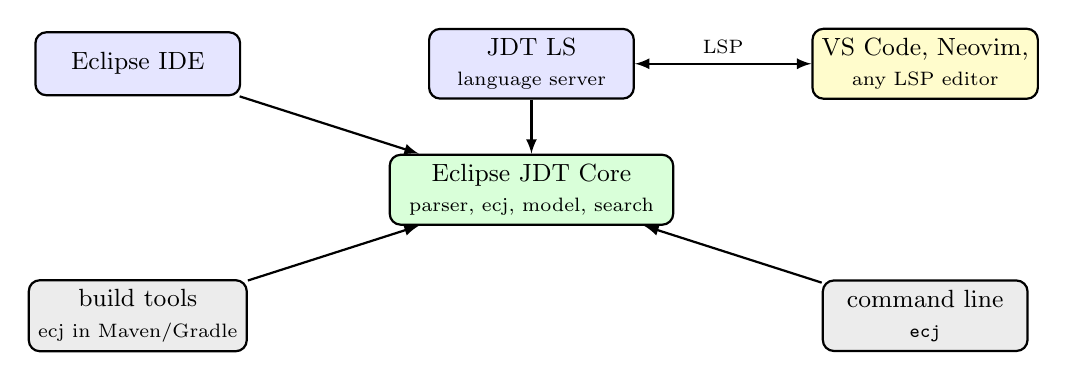
\begin{tikzpicture}[b/.style={draw, thick, rounded corners, minimum width=2.6cm, minimum height=0.8cm, font=\small, align=center}]
    \node[b, fill=green!15, minimum width=3.6cm] (jdt) at (0,0) {Eclipse JDT Core\\ \scriptsize parser, ecj, model, search};
    \node[b, fill=blue!10] (ide) at (-5,1.6) {Eclipse IDE};
    \node[b, fill=blue!10] (ls)  at (0,1.6)  {JDT LS\\ \scriptsize language server};
    \node[b, fill=yellow!20] (vs) at (5,1.6) {VS Code, Neovim,\\ \scriptsize any LSP editor};
    \node[b, fill=gray!15] (mv) at (-5,-1.6) {build tools\\ \scriptsize ecj in Maven/Gradle};
    \node[b, fill=gray!15] (cl) at (5,-1.6)  {command line\\ \scriptsize \texttt{ecj}};
    \draw[-latex, thick] (ide) -- (jdt); \draw[-latex, thick] (ls) -- (jdt); \draw[latex-latex, thick] (vs) -- node[above, font=\scriptsize] {LSP} (ls);
    \draw[-latex, thick] (mv) -- (jdt); \draw[-latex, thick] (cl) -- (jdt);
  \end{tikzpicture}
  \end{center}
  \small The \textbf{Language Server Protocol} separates the editor from the language engine: the same JDT gives
  completion and errors in Eclipse and in VS Code's Java extension.
\end{frame}
% ~~~~~~~~~~~~~~~~~~~~~~~~~~~~~~~~~~~~~~ A frm

% ~~~~~~~~~~~~~~~~~~~~~~~~~~~~~~~~~~~~~~ V
\hSection[Debug info]{What the Debugger Needs}
% ~~~~~~~~~~~~~~~~~~~~~~~~~~~~~~~~~~~~~~ A




% ~~~~~~~~~~~~~~~~~~~~~~~~~~~~~~~~~~~~~~ V frm
\begin{frame}[t,fragile] \frametitle{Debug information in class files}
  \begin{columns}[T]
    \begin{column}{0.38\textwidth}
      \lstcode[basicstyle=\ttfamily\tiny]{codeoutput/DebugInfo/Point.java}{Java}
      \begin{itemize}\small
        \item \texttt{LineNumberTable}: bytecode offset $\to$ source line (breakpoints, stack traces).
        \item \texttt{LocalVariableTable}: names of locals (Variables view).
        \item Eclipse adds both by default (\emph{Java Compiler} preferences).
      \end{itemize}
    \end{column}
    \begin{column}{0.6\textwidth}
      \uncover<2->{\lstterminal[basicstyle=\ttfamily\tiny]{codeoutput/DebugInfo.txt}}
    \end{column}
  \end{columns}
\end{frame}
% ~~~~~~~~~~~~~~~~~~~~~~~~~~~~~~~~~~~~~~ A frm

% ~~~~~~~~~~~~~~~~~~~~~~~~~~~~~~~~~~~~~~ V
\hSection[Team setups]{Reproducible Team Setups}
% ~~~~~~~~~~~~~~~~~~~~~~~~~~~~~~~~~~~~~~ A




% ~~~~~~~~~~~~~~~~~~~~~~~~~~~~~~~~~~~~~~ V frm
\begin{frame}[t,fragile] \frametitle{What a team shares, and how}
  \begin{center}\footnotesize
  \begin{tabular}{@{}L{0.28\textwidth}L{0.42\textwidth}L{0.24\textwidth}@{}}
    \toprule
    \textbf{setting}                    & \textbf{where}                                       & \textbf{share via} \\
    \midrule
    compiler checks, null analysis      & \texttt{.settings/\dots jdt.core.prefs}              & Git \\
    formatter, clean-up, save actions   & \texttt{.settings/\dots jdt.ui.prefs}, profile XML   & Git \\
    launch configurations               & \texttt{*.launch} (\emph{Common} tab: \emph{Shared file}) & Git, \textbf{without secrets} \\
    libraries and Java version          & \texttt{pom.xml} / \texttt{build.gradle}             & Git \\
    IDE, plug-ins, workspace prefs      & Oomph setup file (\texttt{*.setup})                  & Eclipse Installer \\
    \bottomrule
  \end{tabular}
  \end{center}
  \begin{itemize}\small
    \item The build tool is the reference; the IDE settings must agree with it (e.g.\ the same \texttt{release} level).
    \item The CI server compiles with the same rules: \texttt{ecj -properties} with the project's prefs file (junior deck).
    \item \textbf{Oomph}: the Eclipse Installer's advanced mode installs a given IDE, clones the repositories and imports the projects from one file.
  \end{itemize}
\end{frame}
% ~~~~~~~~~~~~~~~~~~~~~~~~~~~~~~~~~~~~~~ A frm




% ~~~~~~~~~~~~~~~~~~~~~~~~~~~~~~~~~~~~~~ V frm
\begin{frame}[t,fragile] \frametitle{A shared launch configuration}
  \lstcode[basicstyle=\ttfamily\tiny]{codeoutput/Grades.launch}{XML}
  \begin{itemize}\small
    \item Plain XML: reviewable and diffable; \emph{Common} tab $\to$ \emph{Shared file} saves it in the project.
    \item \hRemark{Line 8}: an environment variable with a password. Once committed, it is in the history forever (Git deck).
          Use \texttt{\$\{env\_var:DB\_PASSWORD\}} to take it from the developer's environment instead.
  \end{itemize}
\end{frame}
% ~~~~~~~~~~~~~~~~~~~~~~~~~~~~~~~~~~~~~~ A frm

% ~~~~~~~~~~~~~~~~~~~~~~~~~~~~~~~~~~~~~~ V
\hSection[Security]{Security}
% ~~~~~~~~~~~~~~~~~~~~~~~~~~~~~~~~~~~~~~ A




% ~~~~~~~~~~~~~~~~~~~~~~~~~~~~~~~~~~~~~~ V frm
\begin{frame}[t,fragile] \frametitle{An IDE is a powerful program}
  \begin{columns}[T]
    \begin{column}{0.48\textwidth}
      \begin{block}{Plug-ins}
        \small A plug-in runs inside Eclipse with \textbf{your} rights: files, keys, network. Install from known
        update sites only; check who publishes it; p2 warns about \emph{unsigned content}: take it seriously.
      \end{block}
      \begin{block}{Opening a project}
        \small Builders, annotation processors, Maven plug-ins and Gradle scripts \textbf{run code} when a project is
        imported or built. Treat a stranger's project like a stranger's program.
      \end{block}
    \end{column}
    \begin{column}{0.48\textwidth}
      \begin{block}{Debug ports}
        \small \texttt{-agentlib:jdwp} on a reachable port gives full control over the JVM. Bind to \texttt{localhost},
        use an SSH tunnel, never in production.
      \end{block}
      \begin{block}{Secrets}
        \small Not in \texttt{.launch} files, not in \texttt{.settings}, not in the workspace you zip and send.
        Secure storage: \menu{Preferences > General > Security > Secure Storage}.
      \end{block}
    \end{column}
  \end{columns}
\end{frame}
% ~~~~~~~~~~~~~~~~~~~~~~~~~~~~~~~~~~~~~~ A frm

% ~~~~~~~~~~~~~~~~~~~~~~~~~~~~~~~~~~~~~~ V
\hSection[Automation]{Automation and Large Systems}
% ~~~~~~~~~~~~~~~~~~~~~~~~~~~~~~~~~~~~~~ A




% ~~~~~~~~~~~~~~~~~~~~~~~~~~~~~~~~~~~~~~ V frm
\begin{frame}[t,fragile] \frametitle{Eclipse without a window}
  \begin{columns}[T]
    \begin{column}{0.5\textwidth}


% +++++++++++++++++++++++++++++++++++++++ V lst
%: -Lst.
\begin{lstlisting}[style=codesnippet, language={}, basicstyle=\ttfamily\tiny]
eclipse -nosplash -consolelog ^
  -application org.eclipse.jdt.core.JavaCodeFormatter ^
  -config .settings\org.eclipse.jdt.core.prefs src
\end{lstlisting}
% +++++++++++++++++++++++++++++++++++++++ A lst


% +++++++++++++++++++++++++++++++++++++++ V lst
%: -Lst.
\begin{lstlisting}[style=codesnippet, language=bash, basicstyle=\ttfamily\tiny]
./eclipse -nosplash -consolelog \
  -application org.eclipse.jdt.core.JavaCodeFormatter \
  -config .settings/org.eclipse.jdt.core.prefs src
\end{lstlisting}
% +++++++++++++++++++++++++++++++++++++++ A lst


      \small \win{} (Command Prompt) and \mac{} (Terminal, in \texttt{Eclipse.app/Contents/MacOS}).
      \hRemark{Not run here}: needs an Eclipse installation.
    \end{column}
    \begin{column}{0.46\textwidth}
      \begin{itemize}\small
        \item \textbf{Headless applications}: the formatter above formats a whole source tree with the team's settings.
        \item \textbf{Tycho}: builds Eclipse plug-ins and products with Maven.
        \item Large workspaces: close unused projects, use working sets, turn off \emph{Build Automatically} during big
              Git operations, raise \texttt{-Xmx} in \texttt{eclipse.ini}.
      \end{itemize}
    \end{column}
  \end{columns}
\end{frame}
% ~~~~~~~~~~~~~~~~~~~~~~~~~~~~~~~~~~~~~~ A frm




% ~~~~~~~~~~~~~~~~~~~~~~~~~~~~~~~~~~~~~~ V frm
\begin{frame}[t,fragile] \frametitle{Choosing an IDE for a team}
  \begin{center}\small
  \begin{tabular}{L{0.26\textwidth}L{0.66\textwidth}}
    \toprule
    \textbf{criterion}            & \textbf{questions} \\
    \midrule
    build                         & Does the IDE import the Maven/Gradle build without manual steps? \\
    consistency                   & Can compiler checks and formatting be committed and enforced in CI? \\
    extensibility                 & Plug-in API, language servers, scripting? \\
    cost and license              & Free and open (Eclipse: EPL-2.0) or commercial? \\
    resources                     & Memory, start-up time, indexing of large code bases. \\
    \bottomrule
  \end{tabular}
  \end{center}
  \small A team can mix IDEs if the \textbf{build} and the \textbf{checks} live in the repository, not in one IDE's settings.
\end{frame}
% ~~~~~~~~~~~~~~~~~~~~~~~~~~~~~~~~~~~~~~ A frm

% ~~~~~~~~~~~~~~~~~~~~~~~~~~~~~~~~~~~~~~ V
\hSection[Summary]{Summary}
% ~~~~~~~~~~~~~~~~~~~~~~~~~~~~~~~~~~~~~~ A




% ~~~~~~~~~~~~~~~~~~~~~~~~~~~~~~~~~~~~~~ V frm
\begin{frame}[t,fragile] \frametitle{Big ideas}
  \begin{itemize}
    \item Eclipse is a set of OSGi bundles connected by extension points; p2 installs and updates them.
    \item JDT Core (parser, \texttt{ecj}, Java model) is a library: Eclipse, JDT LS (VS Code), build tools and your own programs use it.
    \item The debugger depends on what the compiler writes: line numbers and local variable tables.
    \item Teams commit settings (\texttt{.settings}, \texttt{*.launch}, build files) and check them in CI; Oomph reproduces whole IDEs.
    \item The IDE runs code from plug-ins and projects: trust, signing, secrets and debug ports matter.
  \end{itemize}
\end{frame}
% ~~~~~~~~~~~~~~~~~~~~~~~~~~~~~~~~~~~~~~ A frm




% ~~~~~~~~~~~~~~~~~~~~~~~~~~~~~~~~~~~~~~ V frm
\begin{frame}[t,fragile] \frametitle{Projects}
  \begin{enumerate}\small
    \item \textbf{Mini IDE}: extend \texttt{MiniIde} with a file watcher: recompile on save, print the problems, run tests.
    \item \textbf{Quick fix plug-in}: in the Eclipse SDK, write a quick fix for \texttt{toUpperCase()} without a locale
          (the Turkish \texttt{i} problem).
    \item \textbf{CI parity}: make a GitHub Actions job that compiles with \texttt{ecj -properties .settings/\dots}
          and fails on the same errors as Eclipse.
    \item \textbf{Oomph setup}: one \texttt{.setup} file that installs Eclipse 2026-06 with the course plug-ins
          and imports the course repository; test it on \win{} and \mac.
    \item \textbf{Compare compilers}: find a small program that \texttt{javac} and \texttt{ecj} treat differently; explain
          with the Java Language Specification.
  \end{enumerate}
\end{frame}
% ~~~~~~~~~~~~~~~~~~~~~~~~~~~~~~~~~~~~~~ A frm




% ~~~~~~~~~~~~~~~~~~~~~~~~~~~~~~~~~~~~~~ V frm
\begin{frame}[t,fragile]
	\begin{center}
		\vspace{4cm}
		\hRemark{\Huge Questions?}
	\end{center}
\end{frame}
% ~~~~~~~~~~~~~~~~~~~~~~~~~~~~~~~~~~~~~~ A frm



\end{document}
